\documentclass[conference]{IEEEtran}
\usepackage[T1]{fontenc}
\usepackage{amsmath}
\usepackage{booktabs}
\usepackage{graphicx}
\usepackage{xcolor}
\usepackage{tikz}
\usetikzlibrary{arrows.meta,positioning,calc}
\usepackage{balance}
\usepackage{stfloats}
\usepackage[hidelinks]{hyperref}
\hypersetup{pdftitle={KVFold: Expanding Cache Capacity for LLM Agents with Lossless Compression},
            pdfsubject={ICDE demonstration review draft, version 16}}
\definecolor{fpInk}{HTML}{172634}
\definecolor{fpBlue}{HTML}{1D62D0}
\definecolor{fpTeal}{HTML}{007E6A}
\definecolor{fpOrange}{HTML}{D96C05}
\definecolor{fpPurple}{HTML}{735892}
\tikzset{
  fpbox/.style={draw,rounded corners=2pt,align=center,inner sep=5pt,
                minimum height=0.73cm,line width=0.65pt},
  fparrow/.style={-{Stealth[length=1.7mm]},line width=0.8pt,draw=fpInk},
  fpboth/.style={{Stealth[length=1.7mm]}-{Stealth[length=1.7mm]},
                 line width=0.8pt,draw=fpInk}
}
\title{KVFold: Expanding Cache Capacity for \mbox{LLM Agents} with Lossless Compression}
\author{\IEEEauthorblockN{Working draft}
\IEEEauthorblockA{Author information to be supplied}}
\raggedbottom
\begin{document}
\maketitle

\begin{abstract}
LLM agents often reuse long prompt prefixes when continuing tasks or
resuming sessions. Caching the corresponding key/value (KV) states avoids
repeated prefill, but capacity limits request concurrency and retained
history. KVFold uses lossless
exponent coding to fit more KV into GPU memory and external storage.
Pool mode stores FragPack records on the GPU. Prefill decodes them into
BF16 for FlashAttention-3; decode reconstructs operands within a fused
attention kernel. Tier mode uses a separate record
format in LMCache and leaves the GPU cache layout and attention
implementation unchanged. In recorded AgentX runs with a fixed 54~GiB KV
budget per GPU, pool mode increases usable capacity from 1.18M to 1.59M
tokens. Visitors extend and edit a coding-agent prompt to inspect prefix
reuse and KV reconstruction. They then explore recorded runs to see how
added capacity affects concurrent requests and returning sessions.
\end{abstract}

\section{Introduction}
Consider a coding agent investigating a timeout. Its prompt includes
repository context, a bug report, and the investigation history. If the
user then asks for a regression test, most of the prompt remains unchanged.
Prefix caching avoids repeated prefill by reusing the keys and values
already computed for this shared context. vLLM stores KV in paged
blocks~\cite{vllm}, while LMCache retains
reusable prefixes in DRAM and NVMe across requests~\cite{lmcache}.

For Qwen3-30B-A3B, each cached token requires 96~KiB of BF16 KV across all
layers. With many concurrent sessions, requests may wait for free GPU
blocks even when external storage holds their prefixes. External tiers
relieve GPU memory pressure by storing inactive histories, but can also
fill up. If a resumed session's prefix has been evicted, the engine must
recompute it. Capacity thus limits both concurrency and history reuse.

KVFold uses lossless compression to fit more KV into the available GPU
memory and external storage. The codec preserves each BF16 value's low
byte, assigns short codes to frequent high-byte values, and uses escapes
for the remaining values. Unlike quantization methods such as
KIVI~\cite{kivi} or lossy context codecs such as CacheGen~\cite{cachegen},
it reconstructs the original KV bits. The main \emph{pool mode} stores
completed GPU blocks as FragPack records. During prefill, KVFold gathers
and decodes the context's KV into a BF16 workspace for FlashAttention-3
(FA3)~\cite{fa3}. During decode, it reconstructs operands within a fused
attention kernel. An alternative \emph{tier mode} stores compressed KV in
LMCache while retaining the native GPU cache layout and attention
implementation. Both modes share the coding principle and offline
calibration, but use different formats for attention and external
storage.

The demonstration follows the agent as it continues a task, runs alongside
other sessions, and resumes an earlier investigation. Interactive requests
show prefix reuse, external restoration, and KV byte checks.
Recorded AgentX workloads~\cite{agentx} show the capacity gain at scale:
with a 54~GiB KV budget per GPU, pool mode holds 1.59M tokens compared
with 1.18M for the uncompressed baseline. With admission capped at
12 requests, mean engine time to first token (TTFT) falls from 5.16 to
1.94~s, excluding time spent waiting at the proxy.

\begin{figure*}[t]
\centering
% KVFold architecture, manuscript version 5.
% Topology: industry.pdf, Sections III--VI, and manuscript version 3.
% Native vector primitives; oblique depth denotes pages, chips and devices,
% not measured capacity. Blue = FragPack payload; orange = BF16/attention;
% teal = external-cache devices and tier payload. The lanes are alternatives.
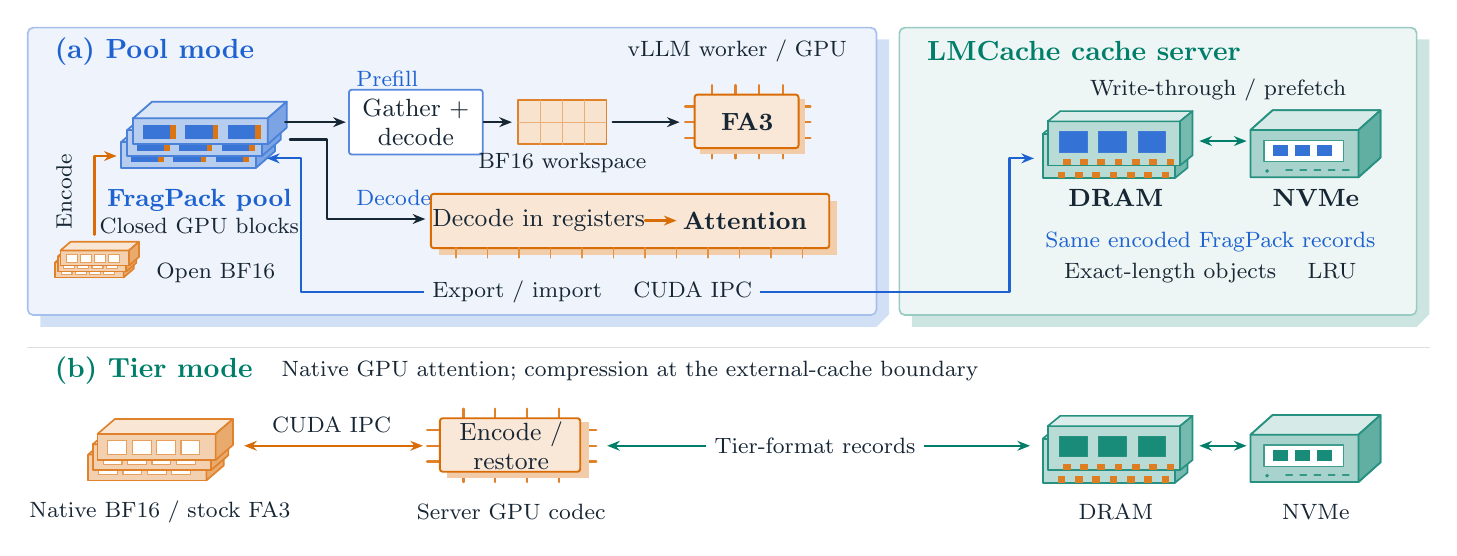
\begin{tikzpicture}[x=1cm,y=1cm,text=fpInk,
    font=\fontsize{9}{10.5}\selectfont,
    line join=round,line cap=round,
    flow/.style={-{Stealth[length=1.6mm,width=1.25mm]},line width=.8pt,draw=fpInk},
    transfer/.style={{Stealth[length=1.6mm,width=1.25mm]}-{Stealth[length=1.6mm,width=1.25mm]},line width=.8pt,draw=fpBlue},
    smalltext/.style={font=\fontsize{8}{9}\selectfont},
    pics/packed/.style={code={
      \foreach \z in {0,.15,.30} {
        \begin{scope}[shift={(.5*\z,\z)}]
          \draw[fpBlue!80,line width=.65pt,fill=fpBlue!32]
            (-.91,-.13) rectangle (.80,.20);
          \draw[fpBlue!80,line width=.65pt,fill=fpBlue!16]
            (-.91,.20) -- (-.67,.41) -- (1.04,.41) -- (.80,.20) -- cycle;
          \draw[fpBlue!80,line width=.65pt,fill=fpBlue!58]
            (.80,-.13) -- (1.04,.08) -- (1.04,.41) -- (.80,.20) -- cycle;
          \foreach \x in {-.79,-.25,.29} {
            \fill[fpBlue!88] (\x,-.06) rectangle +( .35,.17);
            \fill[fpOrange!94] (\x+.35,-.06) rectangle +(.07,.17);
          }
        \end{scope}
      }
    }},
    pics/native/.style={code={
      \foreach \z in {0,.13,.26} {
        \begin{scope}[shift={(.45*\z,\z)}]
          \draw[fpOrange!85,line width=.6pt,fill=fpOrange!32]
            (-.83,-.21) rectangle (.67,.12);
          \draw[fpOrange!85,line width=.6pt,fill=fpOrange!17]
            (-.83,.12) -- (-.61,.31) -- (.89,.31) -- (.67,.12) -- cycle;
          \draw[fpOrange!85,line width=.6pt,fill=fpOrange!58]
            (.67,-.21) -- (.89,-.02) -- (.89,.31) -- (.67,.12) -- cycle;
          \foreach \x in {-.70,-.39,-.08,.23} {
            \draw[fpOrange!65,fill=white,line width=.4pt]
              (\x,-.14) rectangle +(.24,.18);
          }
        \end{scope}
      }
    }},
    pics/chip/.style={code={
      \foreach \x in {-.45,-.15,.15,.45} {
        \draw[fpOrange!85,line width=.9pt] (\x,-.46) -- (\x,-.34);
        \draw[fpOrange!85,line width=.9pt] (\x,.34) -- (\x,.47);
      }
      \foreach \y in {-.20,0,.20} {
        \draw[fpOrange!85,line width=.9pt] (-.79,\y) -- (-.65,\y);
        \draw[fpOrange!85,line width=.9pt] (.65,\y) -- (.80,\y);
      }
      \fill[fpOrange!35] (-.60,-.41) rectangle (.73,.30);
      \draw[fpOrange,line width=.7pt,fill=fpOrange!16,rounded corners=1pt]
        (-.67,-.33) rectangle (.65,.35);
    }},
    pics/dram/.style={code={
      \foreach \z in {0,.16} {
        \begin{scope}[shift={(.40*\z,\z)}]
          \draw[fpTeal!85,line width=.65pt,fill=fpTeal!28]
            (-.84,-.25) rectangle (.84,.31);
          \draw[fpTeal!85,line width=.6pt,fill=fpTeal!14]
            (-.84,.31) -- (-.68,.44) -- (1.0,.44) -- (.84,.31) -- cycle;
          \draw[fpTeal!85,line width=.6pt,fill=fpTeal!54]
            (.84,-.25) -- (1.0,-.12) -- (1.0,.44) -- (.84,.31) -- cycle;
          \foreach \x in {-.69,-.19,.31} {
            \draw[fpPayload!85,line width=.4pt,fill=fpPayload!90]
              (\x,-.08) rectangle +(.35,.26);
          }
          \foreach \x in {-.65,-.43,-.21,.01,.23,.45,.67} {
            \fill[fpOrange!88] (\x,-.25) rectangle +(.10,.08);
          }
        \end{scope}
      }
    }},
    pics/nvme/.style={code={
      \draw[fpTeal!85,line width=.65pt,fill=fpTeal!34]
        (-.72,-.24) -- (.65,-.24) -- (.93,.01) -- (.93,.61)
        -- (-.44,.61) -- (-.72,.36) -- cycle;
      \draw[fpTeal!85,line width=.65pt,fill=fpTeal!16]
        (-.72,.36) -- (-.44,.61) -- (.93,.61) -- (.65,.36) -- cycle;
      \draw[fpTeal!85,line width=.65pt,fill=fpTeal!62]
        (.65,-.24) -- (.93,.01) -- (.93,.61) -- (.65,.36) -- cycle;
      \draw[fpTeal!75,line width=.5pt,fill=white]
        (-.55,-.04) rectangle (.46,.23);
      \foreach \x in {-.44,-.16,.12} {
        \fill[fpPayload!90] (\x,.025) rectangle +(.20,.14);
      }
      \fill[fpTeal!85] (-.51,-.16) circle (.025);
      \foreach \x in {-.27,-.09,.09,.27,.45} {
        \draw[fpTeal!80,line width=.55pt] (\x,-.15) -- +( .08,0);
      }
    }}]
  \path[use as bounding box] (0,0) rectangle (17.8,6.35);
  \colorlet{fpPayload}{fpBlue}

  % Raised host regions: the main reader path stays inside the vLLM worker.
  \fill[fpBlue!20] (.16,2.55) -- (10.78,2.55) -- (10.94,2.71)
    -- (10.94,6.20) -- (.16,6.20) -- cycle;
  \fill[fpBlue!7,draw=fpBlue!40,line width=.6pt,rounded corners=2pt]
    (0,2.70) rectangle (10.78,6.35);
  \fill[fpTeal!20] (11.23,2.55) -- (17.64,2.55) -- (17.80,2.71)
    -- (17.80,6.20) -- (11.23,6.20) -- cycle;
  \fill[fpTeal!7,draw=fpTeal!40,line width=.6pt,rounded corners=2pt]
    (11.07,2.70) rectangle (17.64,6.35);
  \node[anchor=west,font=\fontsize{10}{11}\selectfont\bfseries,text=fpBlue]
    at (.22,6.05) {(a) Pool mode};
  \node[anchor=east,smalltext] at (10.53,6.05) {vLLM worker / GPU};
  \node[anchor=west,font=\fontsize{10}{11}\selectfont\bfseries,text=fpTeal]
    at (11.30,6.05) {LMCache cache server};

  % Persistent compressed records and writable, still-open BF16 storage.
  \pic at (2.10,4.70) {packed};
  \node[font=\fontsize{9}{10}\selectfont\bfseries,text=fpBlue]
    at (2.18,4.16) {FragPack pool};
  \node[smalltext] at (2.18,3.84) {Closed GPU blocks};
  \pic[scale=.58] at (.83,3.30) {native};
  \node[smalltext,anchor=west] at (1.51,3.23) {Open BF16};
  \draw[flow,draw=fpOrange] (.85,3.72) -- (.85,4.72) -- (1.13,4.72);
  \node[smalltext,rotate=90,fill=fpBlue!7,inner sep=2pt]
    at (.46,4.27) {Encode};

  % Prefill explicitly materializes BF16 before unchanged FA3.
  \node[smalltext,text=fpBlue,anchor=west] at (4.05,5.70) {Prefill};
  \draw[flow] (3.27,5.15) -- (4.04,5.15);
  \node[draw=fpBlue!75,fill=white,line width=.65pt,rounded corners=1pt,
    minimum width=1.70cm,minimum height=.64cm,align=center]
    (gather) at (4.93,5.15) {Gather +\\decode};
  \draw[flow] (gather.east) -- (6.15,5.15);
  \draw[fpOrange!85,fill=fpOrange!19,line width=.55pt]
    (6.23,4.87) rectangle (7.35,5.43);
  \foreach \x in {6.51,6.79,7.07}
    \draw[fpOrange!55,line width=.45pt] (\x,4.87) -- (\x,5.43);
  \draw[fpOrange!55,line width=.45pt] (6.23,5.15) -- (7.35,5.15);
  \node[smalltext] at (6.79,4.63) {BF16 workspace};
  \draw[flow] (7.43,5.15) -- (8.28,5.15);
  \pic at (9.14,5.15) {chip};
  \node[font=\fontsize{9}{10}\selectfont\bfseries] at (9.14,5.15) {FA3};

  % The decode alternative reconstructs operands inside the attention kernel.
  \draw[flow] (3.33,4.93) -- (3.80,4.93) -- (3.80,3.92) -- (5.05,3.92);
  \node[smalltext,anchor=west,text=fpBlue] at (4.05,4.19) {Decode};
  \fill[fpOrange!34] (5.22,3.46) rectangle (10.28,4.15);
  \draw[fpOrange,line width=.7pt,fill=fpOrange!17,rounded corners=1pt]
    (5.12,3.55) rectangle (10.18,4.24);
  \foreach \x in {5.44,5.84,6.24,6.64,7.04,7.44,7.84,8.24,8.64,9.04,9.44,9.84}
    \draw[fpOrange!75,line width=.7pt] (\x,3.43) -- (\x,3.55);
  \node at (6.49,3.90) {Decode in registers};
  \draw[flow,draw=fpOrange] (7.84,3.90) -- (8.24,3.90);
  \node[font=\fontsize{9}{10}\selectfont\bfseries] at (9.11,3.90) {Attention};

  % Pool export/import carries the same encoded attention records.
  \draw[transfer] (3.04,4.69) -- (3.47,4.69) -- (3.47,2.99)
    -- (12.47,2.99) -- (12.47,4.69) -- (12.78,4.69);
  \node[smalltext,fill=fpBlue!7,inner sep=3pt]
    at (7.17,2.99) {Export / import \quad CUDA IPC};
  \pic at (13.73,4.69) {dram};
  \pic at (16.25,4.69) {nvme};
  \node[font=\fontsize{9}{10}\selectfont\bfseries] at (13.82,4.19) {DRAM};
  \node[font=\fontsize{9}{10}\selectfont\bfseries] at (16.36,4.19) {NVMe};
  \draw[transfer,draw=fpTeal] (14.88,4.91) -- (15.48,4.91);
  \node[smalltext] at (15.12,5.56) {Write-through / prefetch};
  \node[smalltext,text=fpBlue] at (15.02,3.63) {Same encoded FragPack records};
  \node[smalltext] at (15.02,3.24) {Exact-length objects \quad LRU};

  % Alternative deployment, aligned with the main path's storage devices.
  \colorlet{fpPayload}{fpTeal}
  \draw[fpInk!15,line width=.55pt] (0,2.29) -- (17.8,2.29);
  \node[anchor=west,font=\fontsize{10}{11}\selectfont\bfseries,text=fpTeal]
    at (.22,1.99) {(b) Tier mode};
  \node[smalltext,anchor=west] at (3.10,1.99)
    {Native GPU attention; compression at the external-cache boundary};
  \pic at (1.60,.81) {native};
  \node[smalltext] at (1.68,.20) {Native BF16 / stock FA3};
  \draw[transfer,draw=fpOrange] (2.75,1.04) -- (5.02,1.04);
  \node[smalltext] at (3.86,1.31) {CUDA IPC};
  \pic[xscale=1.35] at (6.14,1.04) {chip};
  \node[align=center] at (6.14,1.04) {Encode /\\restore};
  \node[smalltext] at (6.14,.20) {Server GPU codec};
  \draw[transfer,draw=fpTeal] (7.36,1.04) -- (12.73,1.04);
  \node[smalltext,fill=white,inner sep=3pt] at (10.00,1.04) {Tier-format records};
  \pic at (13.73,.82) {dram};
  \pic at (16.25,.82) {nvme};
  \node[smalltext] at (13.82,.20) {DRAM};
  \node[smalltext] at (16.36,.20) {NVMe};
  \draw[transfer,draw=fpTeal] (14.88,1.04) -- (15.48,1.04);
\end{tikzpicture}

\caption{KVFold's two integration paths. Pool mode stores FragPack records
on the GPU and exports the same records to LMCache. Tier mode keeps the
native GPU cache layout; the cache server encodes and restores KV.
In both modes, LMCache manages storage in DRAM and NVMe, including eviction,
write-through, and prefetch. Completed blocks are encoded; open blocks retain
BF16 values for updates and attention.}
\label{fig:architecture}
\end{figure*}

\section{System Description}
\label{sec:design}
KVFold integrates with vLLM 0.30 and the multiprocess cache server in
LMCache 0.5.6 (Figure~\ref{fig:architecture}). vLLM schedules requests and
allocates 128-token blocks. LMCache handles external lookup, LRU eviction,
write-through, and prefetch.

\subsection{Compressing closed blocks in the GPU pool}
New KV enters a BF16 staging buffer as each block fills. At each
layer, the backend writes the new values, computes attention, and encodes
newly completed blocks. These records remain immutable in the
layer's compressed pool. Incomplete blocks stay in staging so that later
tokens can be appended.

A FragPack record stores one block's K or V for a layer and KV head:
128 tokens with 128 dimensions each, or 32~KiB in BF16. Seven frequent
high-byte values have direct three-bit codes. Other values use a four-bit
escape selector to choose among 15 additional values or fall back to a raw
high byte. K and V use separate tables, calibrated for each layer and KV
head. Low bytes are stored unchanged. Dense streams store scalars in the
order required by the attention kernel's threads
(Figure~\ref{fig:record}).

\begin{figure}[t]
\centering
% Restored worked record example from images/figure2(6).tex.
% Identical scalar values, code assignments, field lengths and alignment.
% Original CPU validation: evidence/record-example.json.
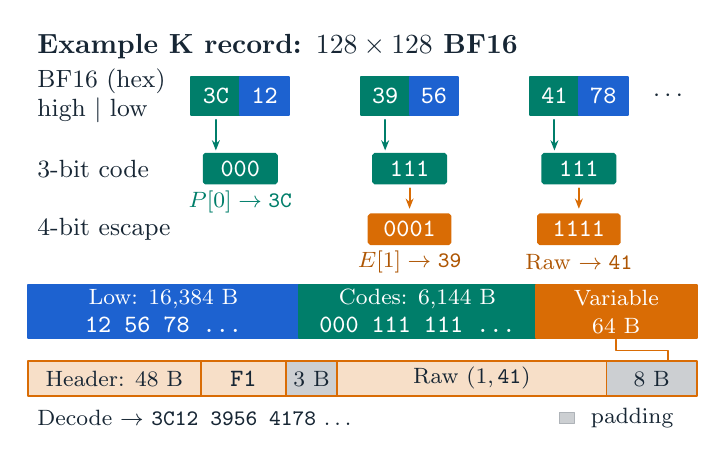
\begin{tikzpicture}[x=1cm,y=1cm,text=fpInk,
    font=\fontsize{9}{10.5}\selectfont,line cap=round,line join=round,
    arrow/.style={-{Stealth[length=1.3mm,width=1mm]},line width=.7pt},
    bits/.style={font=\fontsize{9}{10}\selectfont\ttfamily\bfseries},
    note/.style={font=\fontsize{8.5}{10}\selectfont}]
  \path[use as bounding box] (0,0) rectangle (8.5,5.02);
  \node[anchor=west,font=\fontsize{10}{11}\selectfont\bfseries]
    at (0,4.78) {Example K record: $128\times128$ BF16};

  % Three worked scalars: direct, extended-table and raw escape.
  \node[anchor=west,align=left] at (0,4.15) {BF16 (hex)\\high $\mid$ low};
  \foreach \x/\hi/\lo in {2.70/3C/12,4.85/39/56,7.00/41/78} {
    \draw[fpTeal,fill=fpTeal,line width=.7pt]
      (\x-.62,3.91) rectangle (\x,4.39);
    \draw[fpBlue,fill=fpBlue,line width=.7pt]
      (\x,3.91) rectangle (\x+.62,4.39);
    \node[bits,text=white] at (\x-.31,4.15) {\hi};
    \node[bits,text=white] at (\x+.31,4.15) {\lo};
    \draw[arrow,draw=fpTeal] (\x-.31,3.85) -- (\x-.31,3.46);
  }
  \node[bits] at (8.16,4.15) {$\cdots$};

  \node[anchor=west] at (0,3.23) {3-bit code};
  \foreach \x/\code in {2.70/000,4.85/111,7.00/111} {
    \node[draw=fpTeal,fill=fpTeal,line width=.65pt,
      rounded corners=.7pt,minimum width=.93cm,
      minimum height=.38cm,inner sep=1pt,bits,text=white] at (\x,3.23) {\code};
  }
  \node[note,text=fpTeal] at (2.70,2.81) {$P[0]\to\mathtt{3C}$};

  \node[anchor=west] at (0,2.46) {4-bit escape};
  \foreach \x/\nibble in {4.85/0001,7.00/1111} {
    \draw[arrow,draw=fpOrange] (\x,2.98) -- (\x,2.72);
    \node[draw=fpOrange,fill=fpOrange,line width=.65pt,
      rounded corners=.7pt,minimum width=1.04cm,
      minimum height=.38cm,inner sep=1pt,bits,text=white] at (\x,2.46) {\nibble};
  }
  \node[note,text=fpOrange!80!black] at (4.85,2.05) {$E[1]\to\mathtt{39}$};
  \node[note,text=fpOrange!80!black] at (7.00,2.05) {Raw $\to\mathtt{41}$};

  % Fixed streams show both size and corresponding example data in one band.
  \draw[fpBlue,fill=fpBlue,line width=.7pt]
    (0,1.08) rectangle (3.45,1.75);
  \draw[fpTeal,fill=fpTeal,line width=.7pt]
    (3.45,1.08) rectangle (6.45,1.75);
  \draw[fpOrange,fill=fpOrange,line width=.7pt]
    (6.45,1.08) rectangle (8.50,1.75);
  \node[note,text=white] at (1.725,1.57) {Low: 16,384 B};
  \node[note,text=white] at (4.95,1.57) {Codes: 6,144 B};
  \node[note,text=white,align=center] at (7.475,1.415) {Variable\\64 B};
  \node[bits,text=white] at (1.725,1.25) {12 56 78 \ldots};
  \node[bits,text=white] at (4.95,1.25) {000 111 111 \ldots};

  % Variable-detail pads retain their real byte counts without repeated prose.
  \draw[fpOrange,line width=.6pt] (7.475,1.06) -- (7.475,.92) -- (8.13,.92)
    -- (8.13,.79);
  \draw[fpOrange,fill=fpOrange!22,line width=.65pt]
    (0,.34) rectangle (8.50,.79);
  \fill[fpInk!22] (3.28,.35) rectangle (3.93,.78);
  \fill[fpInk!22] (7.35,.35) rectangle (8.49,.78);
  \foreach \x in {2.20,3.28,3.93,7.35}
    \draw[fpOrange,line width=.5pt] (\x,.34) -- (\x,.79);
  \node[note] at (1.10,.565) {Header: 48 B};
  \node[bits] at (2.74,.565) {F1};
  \node[note] at (3.605,.565) {3 B};
  \node[note] at (5.64,.565) {Raw $(1,\mathtt{41})$};
  \node[note] at (7.925,.565) {8 B};

  \node[anchor=west,note] at (0,.06)
    {Decode $\to$ \texttt{3C12 3956 4178} $\ldots$};
  \fill[fpInk!22,draw=fpInk!35,line width=.4pt] (6.75,-.01) rectangle (6.94,.13);
  \node[anchor=west,note] at (7.03,.06) {padding};
\end{tikzpicture}

\caption{Illustrative FragPack record (not to scale). The three scalars
show direct lookup, an extended-table
escape, and a raw escape. Each raw patch stores an escape's position in
the escape sequence and its original high byte. The variable region uses
64~B in this example, within the format's 2,048~B limit. Recombining the
high and low bytes recovers the original BF16 values exactly.}
\label{fig:record}
\end{figure}

A block's K and V records share a page within each layer. For four KV heads,
a page occupies 190,464~B instead of 262,144~B. The same GPU budget therefore
holds 1.376 times as many pages before accounting for auxiliary backend
buffers. Records that exceed the encoding limit or do not fit in a shared
page are stored uncompressed in overflow slots.

\begin{samepage}
\subsection{Computing attention from compressed KV}
\emph{Prefill with gather + FA3.} When a request extends the context, the
adapter gathers the context's KV into a BF16 workspace, decoding compressed
records and copying values from open blocks. An unmodified FA3 kernel
computes attention from this workspace, which holds the current layer's KV.
Completed blocks remain compressed in each layer's pool.

\end{samepage}

\emph{Decode with fused attention.} For each generated token, a kernel divides
the request's context into page ranges. It prefetches encoded records into
shared memory and reconstructs operands in registers for tensor-core
attention. A final kernel combines partial softmax states across the
ranges. This path avoids writing the decoded context to GPU global memory
and supports decode-only CUDA graph replay. A plugin loads the backend
without changing vLLM's source.

Both paths reconstruct the original KV bits exactly. The console reports
KV byte checks separately from generated text because fused attention and
FA3 can use different reduction orders.

\subsection{Storing KV in LMCache}
Pool mode exports completed attention records from all layers into a
relocatable blob containing dimensions, table identity, and lengths.
LMCache stores each 128-token block at its actual length in DRAM and NVMe.
On import, the server places records in GPU pages and updates their record
tables. Failed validation triggers recomputation. The cache server accesses worker
pools through CUDA IPC to run export and import kernels on the corresponding
GPU, with one synchronization per load request.

\emph{Tier mode} preserves the native GPU cache layout and attention
implementation while compressing external KV. Each chunk contains one
block's KV across all layers. Its per-layer, per-head K/V tables share the
pool's calibration. They use only 14 symbols, seven primary and seven
secondary, compared with FragPack's 22. Values are stored in token order. A
three-bit primary code can escape to a second three-bit code and, if
needed, a literal high byte.
Low bytes remain unchanged. FragPack instead uses fragment order and
four-bit escape selectors.
Grouped indices locate escape streams for groups of eight 256-scalar
tiles. Codebooks are fixed at startup and identified by a table digest.
Chunks exceeding the raw
storage limit remain uncompressed.

Each tensor-parallel (TP) rank stores exact-length objects, aligned to
4~KiB for NVMe direct I/O. Once the step producing the KV finishes, the server
encodes full chunks from native pages into a bounded GPU pool.
A background worker copies and commits the records to DRAM. On load,
compressed records are decoded into destination pages. Raw records and
partially shared leading chunks use a scratch buffer before scattering
into pages. CUDA events order copies,
decoding, and page reuse without host waits on the load path. LMCache uses
stored lengths for NVMe prefetch, allowing the same budget to retain more
history.

\section{Demonstration}
\label{sec:demo}
Visitors follow the timeout investigation through prefix reuse, GPU
capacity limits, and session resumption (Figure~\ref{fig:views}). The console
distinguishes live from recorded data and lists the model, TP degree, KV
type, mode, and cache budgets. Modes and codebooks are fixed at startup;
selectors choose recorded configurations.

\begin{figure*}[!b]
\centering
% Paper-size placement of the unchanged standalone dataflow composition.
% Scale vertical coordinates only: fonts, horizontal scales and data stay fixed.
% Native paper canvas: 178 x 158.4 mm; standalone remains 178 x 180 mm.
\begingroup
\tikzset{every picture/.append style={yscale=0.88}}
% Independent data-flow Figure 3; not imported by the version-15 manuscript.
% Native canvas: 178 x 180 mm. Numeric values retain their archived scopes.
% Palette reference: RUBEN, ICDE 2026 Demo, page 2 (local author PDF).
% Four-row flow is schematic, based on the saved November 8 Qwen3-4B run.
% Copy is write-through: GPU records remain resident, not a destructive offload.
% Append uses the GPU prefix (code + continuous run logs), then saves one new block.
% Edit early uses the original prompt with Python changed to TypeScript.
% Restore resets GPU APC and imports the original prefix from LMCache DRAM.
% The Inspector is an independent After Build check, not Restore verification.
% Model, run configuration and explanatory text are in the standalone caption.
\begingroup
\definecolor{viewInk}{HTML}{212121}
\definecolor{viewRaw}{HTML}{747474}
\definecolor{viewBlue}{HTML}{2B76D1}
\definecolor{viewOrange}{HTML}{FE8001}
\definecolor{viewOrangeInk}{HTML}{AD5200}
\definecolor{viewLine}{HTML}{DADADA}
\definecolor{viewBlueFill}{HTML}{DAE8FC}
\definecolor{viewOrangeFill}{HTML}{FFE6CC}
\begin{tikzpicture}[x=1cm,y=1cm,text=viewInk,
  font=\fontsize{10.5}{12}\selectfont,line cap=round,line join=round,
  every node/.style={inner sep=0pt},
  title/.style={font=\fontsize{13}{15}\selectfont\bfseries},
  note/.style={font=\fontsize{9.5}{11}\selectfont},
  label/.style={font=\fontsize{10.5}{12}\selectfont\bfseries},
  metric/.style={font=\fontsize{11.5}{13}\selectfont\bfseries},
  card/.style={draw=viewLine,fill=white,rounded corners=2pt,line width=.6pt},
  transfer/.style={-{Stealth[length=1.9mm,width=1.4mm]},line width=1pt},
  request/.style={-{Stealth[length=1.5mm,width=1.1mm]},
    densely dashed,line width=.6pt,draw=viewInk!55}]
  \path[use as bounding box] (0,0) rectangle (17.8,18.0);

  % (a) Prompt, GPU/DRAM data flow, and saved output; no simulated migration.
  \draw[viewInk!45,fill=white,rounded corners=2pt,line width=.65pt]
    (.05,8.05) rectangle (17.75,17.95);
  \fill[viewBlue,rounded corners=2pt] (.07,17.30) rectangle (17.73,17.93);
  \node[title,text=white,anchor=west] at (.35,17.625) {(a) Prefix reuse};

  % Verbatim prompt and code excerpts, in a compact shared input card.
  \draw[card] (.35,15.92) rectangle (17.45,17.10);
  \node[label,anchor=west] at (.60,16.52) {Prompt};
  \node[note,anchor=west] at (2.10,16.78)
    {You are maintaining a Python repository.};
  \node[note,anchor=west] at (2.10,16.32)
    {Diagnose the timeout failure below.};
  \node[anchor=west,font=\fontsize{9}{11}\selectfont\ttfamily]
    at (10.05,16.78) {deadline = monotonic() + timeout};
  \node[anchor=west,font=\fontsize{9}{11}\selectfont\ttfamily]
    at (10.05,16.32) {connection = await client.acquire()};

  % Shared lanes. The small rectangles are closed 128-token prefix blocks;
  % their width is schematic, not a byte-size or wall-clock scale.
  \fill[viewBlueFill!40,rounded corners=2pt] (4.55,10.32) rectangle (9.65,15.75);
  \fill[viewOrangeFill!50,rounded corners=2pt] (12.00,10.32) rectangle (17.45,15.75);
  \node[label,anchor=west] at (.60,15.45) {Action};
  \node[label,text=viewBlue] at (7.10,15.45) {GPU KV};
  \node[label,text=viewOrangeInk] at (14.725,15.45) {LMCache DRAM};

  \foreach \y/\n/\action/\detail/\result/\gpuOp/\hostLabel/\blocks in {
    14.68/1/Build/{Original prompt}/{534 computed}/{Encode 4 closed blocks}/{4 original-prefix blocks}/4,
    13.43/2/Append/{Add a regression test}/{512 reused + 144 computed}/{Encode 1 new block}/{+1 new suffix block}/1,
    12.18/3/{Edit early}/{``Python'' $\rightarrow$ ``TypeScript''}/{0 reused + 534 computed}/{Encode 4 new blocks}/{+4 edited-prefix blocks}/4,
    10.93/4/Restore/{Replay original prompt}/{512 restored + 22 computed}/{After GPU cache reset}/{4 original-prefix blocks}/4} {
    \ifnum\n=4
      \draw[viewBlue,fill=viewBlue,rounded corners=2pt,line width=.6pt]
        (.35,\y-.48) rectangle (4.15,\y+.48);
      \node[label,text=white] at (2.25,\y+.18) {\n.\ \action};
      \node[note,text=white] at (2.25,\y-.21) {Replay original prompt};
    \else
      \draw[card] (.35,\y-.48) rectangle (4.15,\y+.48);
      \node[label] at (2.25,\y+.18) {\n.\ \action};
      \node[note] at (2.25,\y-.21) {\detail};
    \fi
    \draw[request] (4.27,\y) -- (4.67,\y);
    \draw[card] (4.80,\y-.48) rectangle (9.40,\y+.48);
    \node at (7.10,\y+.18) {\result};
    \node[note,text=viewBlue] at (7.10,\y-.23) {\gpuOp};
    \draw[card] (12.25,\y-.48) rectangle (17.20,\y+.48);
    \node[note] at (14.725,\y+.18) {\hostLabel};
    \pgfmathsetmacro{\recordLeft}{14.725-(.45*\blocks+.12*(\blocks-1))/2}
    \foreach \k in {1,...,\blocks} {
      \pgfmathsetmacro{\recordX}{\recordLeft+.57*(\k-1)}
      \fill[viewBlue!18] (\recordX+.05,\y-.30) rectangle +(.45,.22);
      \draw[viewBlue,fill=viewBlue!70,line width=.4pt]
        (\recordX,\y-.25) rectangle +(.45,.22);
    }
    \ifnum\n=4
      \draw[transfer,viewOrange] (11.80,\y) -- (9.85,\y);
      \node[note,text=viewOrangeInk] at (10.825,\y+.27) {Import};
    \else
      \draw[transfer,viewBlue] (9.85,\y) -- (11.80,\y);
      \node[note,text=viewBlue] at (10.825,\y+.27) {Copy};
    \fi
  }

  % The output is an exact fragment from the recorded Restore response.
  \draw[card] (.35,8.25) rectangle (10.95,9.95);
  \node[label,anchor=west] at (.60,9.61) {Restore response};
  \node[anchor=north west,text width=9.85cm,align=left,
    font=\fontsize{10.5}{12.5}\selectfont] at (.60,9.20)
    {``\ldots it is not enforced during the \texttt{client.acquire()} call.''};
  \node[anchor=west] at (.60,8.62) {TTFT \textbf{47.3 ms}};

  % Independent inspector aligns with the response card within panel (a).
  \fill[viewInk!8,rounded corners=2pt] (11.33,8.17) rectangle (17.53,9.87);
  \draw[viewInk!35,fill=white,rounded corners=2pt,line width=.6pt]
    (11.25,8.25) rectangle (17.45,9.95);
  \fill[viewBlueFill!35,rounded corners=2pt] (11.27,9.37) rectangle (17.43,9.93);
  \node[label,anchor=west] at (11.50,9.61) {KV Inspector (Build)};
  \node[metric] at (12.75,9.10) {18.00 MiB};
  \draw[transfer,viewBlue] (13.97,9.10) -- (14.50,9.10);
  \node[metric] at (15.88,9.10) {12.73 MiB};
  \node at (14.35,8.57)
    {\textcolor{viewBlue}{\textbf{0}} BF16 mismatches};

  % (b)(c) No row gridlines. Rendered glyph bounds give approximately 2 mm
  % of optical padding at both column ends; type sizes are unchanged.
  \foreach \bottom/\top/\col/\tint in {
    4.05/7.60/viewBlue/viewBlueFill,.05/3.60/viewOrange/viewOrangeFill} {
    \draw[viewInk!45,fill=white,rounded corners=2pt,line width=.6pt]
      (.05,\bottom) rectangle (17.75,\top);
    \fill[\tint!50,rounded corners=2pt]
      (.07,\top-.65) rectangle (17.73,\top-.02);
    \fill[viewInk!3,rounded corners=2pt]
      (5.65,\bottom+.16) rectangle (11.40,\top-.79);
    \fill[\tint!30,rounded corners=2pt]
      (11.70,\bottom+.16) rectangle (17.45,\top-.79);
    \node[label] at (8.525,\top-1.122) {Raw};
  }
  \node[title,anchor=west] at (.35,7.275) {(b) GPU capacity};
  \node[label,anchor=west] at (.35,6.478) {54 GiB KV / GPU};
  \node[label,text=viewBlue] at (14.575,6.478) {Pool mode};
  \node[title,anchor=west] at (.35,3.275) {(c) History retention};
  \node[label,anchor=west] at (.35,2.478) {400 GiB DRAM};
  \node[label,text=viewOrangeInk] at (14.575,2.478) {Tier mode};

  % Shared per-metric scales. Raw 100% is the normalized raw/raw baseline.
  \foreach \y/\lab/\dir/\raw/\compressed/\maximum/\rawText/\compressedText/\col in {
    5.863/{KV tokens per GPU}/\uparrow/1.18/1.59/1.6/1.18M/1.59M/viewBlue,
    5.248/{Waiting requests (mean)}/\downarrow/1.5/.4/2.0/1.5/0.4/viewBlue,
    4.633/{Engine TTFT (s)}/\downarrow/5.16/1.94/7.0/5.16/1.94/viewBlue,
    1.863/{Cached tokens (GPU + ext.)}/\uparrow/55/91/100/{55\%}/{91\%}/viewOrange,
    1.248/{Stored / raw bytes}/\downarrow/100/71.6/100/{100\%}/{71.6\%}/viewOrange,
    .633/{Engine TTFT (s)}/\downarrow/6.76/2.34/7.0/{6.76\phantom{\%}}/{2.34\phantom{\%}}/viewOrange} {
    \node[anchor=west] at (.35,\y) {\lab};
    \node[text=viewInk!70] at (5.23,\y) {$\dir$};
    \fill[viewInk!6] (5.90,\y-.125) rectangle +(3.80,.25);
    \fill[\col!9] (11.95,\y-.125) rectangle +(3.80,.25);
    \draw[viewRaw,fill=viewRaw!70,line width=.4pt]
      (5.90,\y-.125) rectangle +({3.80*\raw/\maximum},.25);
    \draw[\col,fill=\col!78,line width=.4pt]
      (11.95,\y-.125) rectangle +({3.80*\compressed/\maximum},.25);
    \node[metric,anchor=east] at (11.15,\y) {\rawText};
    \node[metric,anchor=east] at (17.20,\y) {\compressedText};
  }
\end{tikzpicture}
\endgroup

\endgroup

\caption{Recomposed views. (a) Saved Qwen3-4B session.
Dashed arrows mark requests; GPU--DRAM arrows transfer compressed blocks.
Copy retains GPU records. Inspector: BF16/blob sizes and independent
export/import after Build (576 records).
(b,c) Archived Qwen3-30B AgentX: $P=64$, 400~GiB DRAM;
(b) $S=12$, 2~TiB NVMe; (c) $S=8$, 640~GiB NVMe.
Paired bars share scales; cached tokens include GPU/external hits;
raw bytes are normalized to 100\%.}
\label{fig:views}
\end{figure*}

\emph{Setup.} The interactive session runs Qwen3-4B-Instruct-2507 in eager
pool mode on one H800 PCIe GPU. It uses BF16 weights and KV, TP 1,
128-token blocks, a 4~GiB GPU KV budget, and 1~GiB of LMCache DRAM.

The recorded capacity experiments used Qwen3-30B-A3B-Instruct
with FP8 weights and BF16 KV, TP 2, and two H800 SXM GPUs connected over
PCIe. vLLM used 128-token blocks and 8,192-token chunked prefill.
AgentX harness 1.0.7 replayed \texttt{cc\_traces\_weka\_062126\_256k} using
seed 42 and the recorded think times. $P$ counts live root sessions; a FIFO
proxy admits at most $S$ concurrent requests. Measurements covered
1,800 seconds after priming and ten warmup requests. Requests without a
first token by the end of the window were excluded. \emph{Engine TTFT} excludes
proxy wait. \emph{Goodput} counts requests/minute with engine TTFT at most
2~s and inter-token latency (ITL) at most 40~ms.
% Current codec description: feat/lmcache-056-lossless-kv at d096273.
% Recorded measurements: main(11).pdf, November 4, 2026; exact run commits
% are not identified in the supplied report.
These measurements and output checks predate the shared calibration and
grouped index described in Section~\ref{sec:design}. The recorded tier runs
used per-plane codebooks and the earlier tile index.

\subsection{Step 1: extend a task and inspect prefix reuse}
Visitors use \emph{Build} to submit repository context, a bug report,
and ``Diagnose the timeout failure.'' They then use \emph{Append} to add
``Write a regression test.'' A prefix strip shows reused and new tokens
alongside cached-token counts, TTFT, and the model's response.
\emph{Edit early} limits reuse to complete
128-token blocks before the changed token.

\emph{Restore} waits for external saves, resets the GPU prefix cache, and
replays the original prompt. The saved session restored 512 tokens from
LMCache DRAM.

The inspector compares decoded KV from an already encoded block before
and after export through host memory and import into an independent GPU
scratch store. It displays sizes, checksums, and mismatch counts. All layers
of the captured 128-token block matched byte for byte. Separate CPU samples
exercise escapes and raw fallback.

A historical check found identical greedy outputs for 192 repeat-trace
requests in tier and raw-tier modes with matching execution paths.

\subsection{Step 2: explore GPU capacity limits}
Visitors select $S=8$ or $S=12$ to compare raw and pool modes under equal
GPU KV budgets (Table~\ref{tab:gpu}). External tiers retain the working set,
with a cached-token share of 0.94 in all runs. These runs examine GPU
pressure when prefixes are cached.

% Source: main(11).pdf, p.10, Table V; printed values retained verbatim.
\begin{table}[t]
\centering
\caption{GPU capacity and performance in the recorded runs: 54 GiB KV per
GPU, $P=64$, 400 GiB DRAM, and 2 TiB NVMe. Wait denotes the mean number of
requests waiting in vLLM; TTFT is mean engine TTFT in seconds.}
\label{tab:gpu}
\small
\setlength{\tabcolsep}{3pt}
\begin{tabular*}{\columnwidth}{@{\extracolsep{\fill}}rlrrrr@{}}
\toprule
$S$ & Mode & KV tokens & Wait & TTFT & Goodput \\
\midrule
8  & Raw  & 1.18M & 0.3 & 1.69 & 15.1 \\
8  & Pool & 1.59M & 0.2 & 1.34 & 16.2 \\
12 & Raw  & 1.18M & 1.5 & 5.16 & 10.6 \\
12 & Pool & 1.59M & 0.4 & 1.94 & 14.9 \\
\bottomrule
\end{tabular*}
\end{table}

Pool mode reserves 1.3~GiB within the KV budget for staging, overflow, and
the prefill workspace. Cache-server CUDA contexts and transfer buffers are
accounted for separately; codec buffers occupy 1.0~GiB per GPU outside
vLLM's budget.

At $S=12$, pool mode keeps TTFT close to raw mode at $S=8$.
At the higher cap, pool mode has fewer waiting requests and higher goodput
than raw mode.

\subsection{Step 3: revisit sessions under storage pressure}
Visitors select 640~GiB or 2~TiB NVMe to compare retained
history, stored bytes, TTFT, and goodput (Table~\ref{tab:tiers}). Raw and tier
modes share the native GPU KV layout, FA3, and LMCache's LRU, write-through,
and prefetch policies. They allocate different record sizes.

% Source: main(11).pdf, p.9, Table III; same P/S and metric definitions.
\begin{table}[t]
\centering
\caption{External cache capacity and performance in the recorded runs:
$P=64$, $S=8$, and 400 GiB DRAM. Cached denotes the share of prompt tokens
served from the GPU or external cache; TTFT is mean engine TTFT in seconds.}
\label{tab:tiers}
\small
\setlength{\tabcolsep}{3pt}
\begin{tabular*}{\columnwidth}{@{\extracolsep{\fill}}llrrr@{}}
\toprule
NVMe & Mode & Cached & TTFT & Goodput \\
\midrule
640 GiB & Raw  & 0.55 & 6.76 & 4.6 \\
640 GiB & Tier & 0.91 & 2.34 & 13.5 \\
2 TiB   & Raw  & 0.94 & 1.69 & 15.1 \\
2 TiB   & Tier & 0.94 & 1.85 & 15.4 \\
\bottomrule
\end{tabular*}
\end{table}

At 640~GiB NVMe, tier mode's compressed-to-raw size ratio of 0.716 allows
about 1.4 times as much KV to fit (Figure~\ref{fig:views}(c)). At 2~TiB, the raw
working set fits and cached-token shares converge (Table~\ref{tab:tiers}).
Input throughput in tier mode is then 26.9 thousand tokens/s versus 27.5
for raw storage, a 2.2\% reduction.

A separate replay of 48 prompts, with one request in flight, compares DRAM
and NVMe hits. The prompts' KV occupies 261~GiB raw and 188~GiB compressed. At
220~GiB DRAM, compressed KV fits in memory, while some raw prefixes require
NVMe reads. For 8K--128K prompts, mean warm TTFT with raw storage is
1.63--1.68 times that of tier mode. At 400~GiB DRAM, both representations
fit and the gap narrows.
The console displays these recorded residency and latency comparisons.

\section{Conclusion}
KVFold fits more KV into GPU memory and external cache tiers. Visitors
inspect prefix reuse, restore KV from LMCache, and check a model block
before and after transfer. Recorded comparisons show how the additional
capacity affects request queues and history reuse under fixed budgets.

\section*{Acknowledgment}
% To be completed by the authors.

\bibliographystyle{IEEEtran}
\bibliography{references}
\end{document}
